\documentclass[12pt,a4paper]{article}
\usepackage{ctex}
\usepackage{amsmath,amscd,amsbsy,amssymb,latexsym,url,bm,amsthm}
\usepackage{epsfig,graphicx,subfigure}
\usepackage{enumitem,balance}
\usepackage{wrapfig}
\usepackage{mathrsfs,euscript}
\usepackage[usenames]{xcolor}
\usepackage{hyperref}
\usepackage[vlined,ruled,linesnumbered]{algorithm2e}
\hypersetup{colorlinks=true,linkcolor=black}

\newtheorem{theorem}{Theorem}
\newtheorem{lemma}[theorem]{Lemma}
\newtheorem{proposition}[theorem]{Proposition}
\newtheorem{corollary}[theorem]{Corollary}
\newtheorem{exercise}{Exercise}
\newtheorem*{solution}{Solution}
\newtheorem{definition}{Definition}
\theoremstyle{definition}

\renewcommand{\thefootnote}{\fnsymbol{footnote}}

\newcommand{\postscript}[2]
 {\setlength{\epsfxsize}{#2\hsize}
  \centerline{\epsfbox{#1}}}

\renewcommand{\baselinestretch}{1.0}

\setlength{\oddsidemargin}{-0.365in}
\setlength{\evensidemargin}{-0.365in}
\setlength{\topmargin}{-0.3in}
\setlength{\headheight}{0in}
\setlength{\headsep}{0in}
\setlength{\textheight}{10.1in}
\setlength{\textwidth}{7in}
\makeatletter \renewenvironment{proof}[1][Proof] {\par\pushQED{\qed}\normalfont\topsep6\p@\@plus6\p@\relax\trivlist\item[\hskip\labelsep\bfseries#1\@addpunct{.}]\ignorespaces}{\popQED\endtrivlist\@endpefalse} \makeatother
\makeatletter
\renewenvironment{solution}[1][Solution] {\par\pushQED{\qed}\normalfont\topsep6\p@\@plus6\p@\relax\trivlist\item[\hskip\labelsep\bfseries#1\@addpunct{.}]\ignorespaces}{\popQED\endtrivlist\@endpefalse} \makeatother

\begin{document}

\noindent

%========================================================================
\noindent\framebox[\linewidth]{\shortstack[c]{
\Large{\textbf{Lab08-Graph Exploration}}\vspace{1mm}\\
CS214-Algorithm and Complexity, Xiaofeng Gao, Spring 2020.}}
\begin{center}
\footnotesize{\color{red}$*$ If there is any problem, please contact TA Yiming Liu.}

% Please write down your name, student id and email.
\footnotesize{\color{blue}$*$ Name:Yijia Diao  \quad Student ID:518030910146 \quad Email: diao\_yijia@sjtu.edu.cn}
\end{center}

\begin{enumerate}
    \item
    \textbf{BFS Tree.} Similar to DFS, BFS yields a tree, (also possibly forest, but \textbf{just consider a tree} in this question) and we can define \textbf{tree, forward, back, cross} edges for BFS. Denote $Dist(u)$ as the distance between node $u$ and the source node in the BFS tree. Please prove:
    \begin{enumerate}
    	\item For both undirected and directed graphs, no forward edges exist in the graph.
    	
    	\item There are no back edges in undirected graph, while in directed graph each back edge $(u,v)$ yields $0\leq Dist(v)\leq Dist(u)$.
    	
    	\item For undirected graph, each cross edge $(u,v)$ yields $|Dist(v)-Dist(u)|\le 1$, while for directed graph, each cross edge $(u,v)$ yields $Dist(v)\leq Dist(u)+1$.
    	
    \end{enumerate}
    
    \begin{proof}
        \begin{enumerate}
        	\item (By contradiction) Suppose there is a forward edge $ (u,v) $, then since $ u $ is connected with $ v $, for undirected graph: $ |Dist(v) - Dist(u)| = 1 $, for directed graph: $ Dist(v) - Dist(u) = 1 $. According to the definition of  forward edge, for directed and undirected graph, we have $ |Dist(v) - Dist(u)| > 1 $, contradiction.\\So we can conclude that for both undirected and directed graphs, no forward edges exist in the graph.
        	\item (By contradiction) \\
        	1. For undirected graph: Suppose there is a back edge $ (u,v) $, then since $ u $ is connected with $ v $, we have $ Dist(u) - Dist(v) = 1 $. According to the definition of back edge, $ Dist(u) < Dist(v) $, contradiction.\\
        	2. For directed graph: Suppose $ Dist(v)>Dist(u) $, then $ v $ is a child or descendant of $ u $. According to the definition of back edge, $ v $ is an ancestor of $ u $, contradiction.\\
        	Therefore we can conclude that the proposition is true.
        	\item (By contradiction) \\
        	1. For undirected graph: Suppose that $|Dist(v)-Dist(u)|> 1$. According to the form of BFS tree, the edge $ (u,v) $ does not exist in the source graph, which leads to contradiction.\\
        	2. For directed graph: Suppose $ Dist(v)> Dist(u)+1 $. According to the form of BFS tree, the edge $ (u,v) $ does not exist in the source graph, which leads to contradiction.\\
        	Therefore we can conclude that the proposition is true.
        \end{enumerate}
    \end{proof}

    \item 
    \textbf{Articulation Points, Bridges, and Biconnected Components.} Let $G=(V, E)$ be a connected, undirected graph. An articulation point of $G$ is a vertex whose removal disconnects $G$. A bridge of $G$ is an edge whose removal disconnects $G .$ A biconnected component of $G$ is a maximal set of edges such that any two edges in the set lie on a common simple cycle. Figure\ref{def} illustrates these definitions. We can determine articulation points, bridges, and biconnected components using depth-first search. Let $G_{\pi}=\left(V, E_{\pi}\right)$ be a depth-first tree of $G$. Please prove:
    
    \begin{enumerate}
    	\item The root of $G_{\pi}$ is an articulation point of $G$ if and only if it has at least two children in $G_{\pi}$.
    	\item\label{2.(b)} An edge of $G$ is a bridge if and only if it does not lie on any simple cycle of $G$.
    	\item The biconnected components of $G$ partition the nonbridge edges of $G$.
    \end{enumerate}

	 \begin{figure}[htbp]
	 	
		\centering
		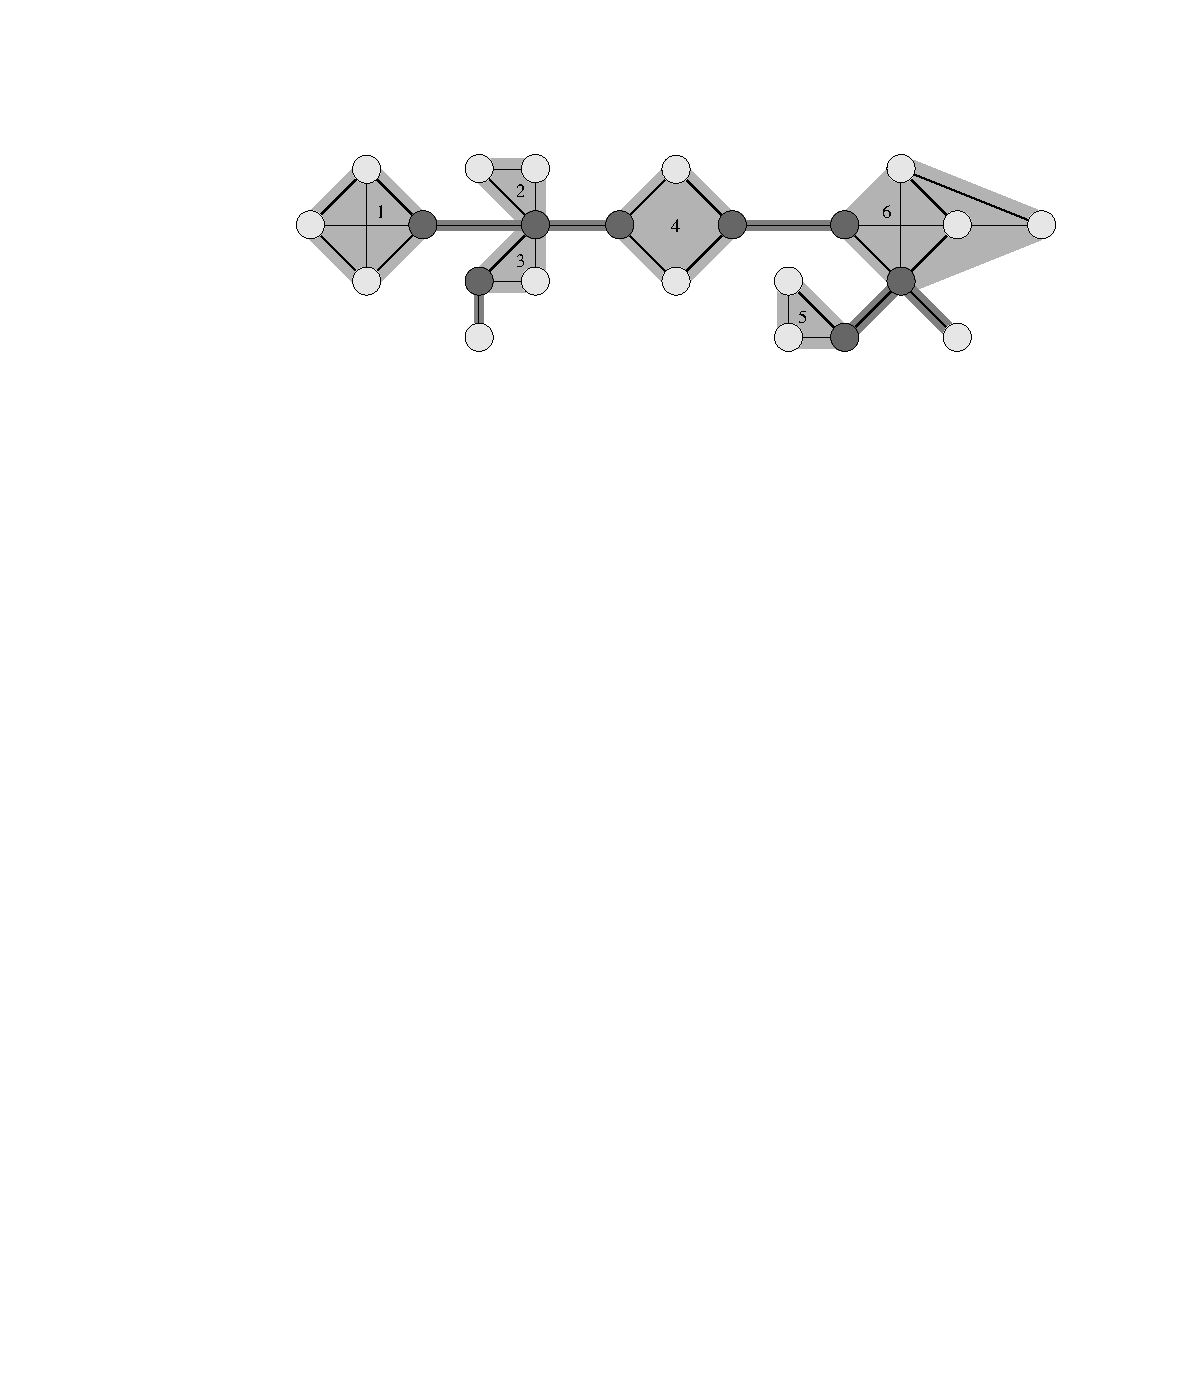
\includegraphics[width=6in]{Fig-Definition.pdf}
		\caption{The definition of articulation points, bridges, and biconnected components. The articulation points are the heavily shaded vertices, the bridges are the heavily shaded edges, and the biconnected components are the edges in the shaded regions, with a \textit{bcc} numbering shown.}
		\label{def}
	\end{figure}
	
	\begin{proof}
		\begin{enumerate}
			\item 
			\begin{lemma}\label{lemma1}
				$\forall u,v\in $DFS tree, $ u $ and $ v $ are connected.
			\end{lemma}
			We have proved the lemma in class.\\
			"$ \Rightarrow $" (By contradiction) Suppose the root of $ G_{\pi} $ has less than 2 children.\\
			1. 0 child: the root doesn't connect to any other vertex. Contradiction with $ G $ is a  connected graph.\\
			2. 1 child: since with the removal of the root, its children is the new root of DFS tree, which indicates that the children is connected with all other nodes, according to Lemma \ref{lemma1}. Therefore the graph is still connected. Contradiction with the definition of the articulation point.
			
			"$ \Leftarrow $" (By contradiction) Suppose the root is not an articulation point, which means if removes it $ G $, the graph is still connected. Then remove it from  $G_{\pi} $, then we have at least 2 new DFS tree, among whom are not connected, which indicates that the remaining nodes of $ G $ are not connected, according to Lemma \ref{lemma1}. Contradiction.
			
			Therefore, we can conclude that the proposition is true.
			\item "$ \Rightarrow $" (By contradiction) Suppose the bridge edge $ (u,v) $ lies on a cycle of $ G $. Then remove edge $ (u,v) $, $ u $ and $ v $ are still connected because of the cycle path. And we do not change other edges, so the connection of all other node pair does not changes, which means $ G $ is connected. Contradiction.
			
			"$ \Leftarrow $" (By contradiction) Suppose the edge $ (u,v) $ is not a bridge. Then remove edge $ (u,v) $, since $ u $ and $ v $ are not on any cycle, then $ u $ and $ v $ are not connected, contradiction with the definition of bridge.
			
			Therefore, we can conclude that the proposition is true.
			\item 1. According to the proposition in (b) , the bridge edges do not lie in any biconnected component.
			
			2. Now prove that the biconnected components is the partition of $ G\backslash \{ \text{bridge edges}\}$.\\
			(\textbf{1}) Disjoint.\\ (By contradiction) Suppose that $ E_{1} $, $ E_{2} $ are two biconnected components, and $ E_{1}\ne E_{2}$,  $E_{1}\cap E_{2}\ne\emptyset$. Then we have edge $ (u,v)$: $(u,v)\in E_{1}\cap E_{2} $. Then $ (u,v) $ and any other edges $ \in E_{1}\cup E_{2}$ lie in a common simple cycle.\\
			Assume that $ E_{1}\backslash E_{2}\ne\emptyset $ (equals to $ E_{2}\backslash E_{1} $'s case). Then $ \forall\text{ edge }(u_{1},v_{1})\in E_{1}\backslash E_{2} $, $ \forall\text{ edge }(u_{2},v_{2})\in E_{2} $, we can find cycle (a set of edges) $ C_{1}: (u_{1},v_{1}),(u,v)\in C_{1} $, $ C_{2}: (u_{2},v_{2}),(u,v)\in C_{2} $. Then consider $ C_{1}\cup C_{2}\backslash(u,v) $, which means the set of two different paths between $ u $ and $ v $, thus $ C_{1}\cup C_{2}\backslash(u,v) $ is also a cycle. So $ (u_{1},v_{1}) , (u_{2},v_{2})\in E_{2} $, which leads to contradiction.\\
			So we can conclude that $ E_{1}\cap E_{2}=\emptyset $\\
			(\textbf{2}) $ \forall E\text{ is biconnected components: }\cup E = G\backslash \{ \text{bridge edges}\} $.\\ 
			(By contradiction) Suppose that there is an edge $ (u,v)\in G $ that does not lie in any biconnected component, also isn't a bridge. Then according to the proposition \ref{2.(b)}, $ (u,v) $ lies on a simple cycle of $G$, and we can find another edge $ (u',v') $ on the same cycle. Then $ \exists \text{ cycle }C: (u,v),(u',v') \in C $, which means $ (u,v) $ lies on a biconnected component, contradiction.\\
			So we can conclude: $ \forall E\text{ is biconnected components: }\cup E = G\backslash \{ \text{bridge edges}\} $
		\end{enumerate}
	\end{proof}

    \item
    Suppose $G=(V, E)$ is a \textbf{Directed Acyclic Graph} (DAG) with positive weights $w(u, v)$ on each edge. Let $s$ be a vertex of $G$ with no incoming edges and assume that every other node is reachable from $s$ through some path.
    
    \begin{enumerate}
    	\item
    	Give an $O(|V|+|E|)$-time algorithm to compute the shortest paths from $s$ to all the other vertices in $G$. Note that this is faster than Dijkstra's algorithm in general.
    	\item
    	Give an efficient algorithm to compute the longest paths from $s$ to all the other vertices.
    \end{enumerate}
    
    \begin{solution}
        \begin{enumerate}
            \item The algorithm below uses the method framed by BFS, and its time complexity is $ O(|V|+|E|) $. Since it does not use the operation of EXTRACT-MIN and DECREASE-KEY, it's faster than Dijkstra's algorithm.\\
            \begin{minipage}[t]{0.89\textwidth}
				\begin{algorithm}[H]
					\KwIn{$G=(V,E), w(u,v), s$.}
					\KwOut{An array of the shortest distance $ d[|V|] $ from $ s $ to all the other vertices in $ G $.}
					\BlankLine
					\caption{Shortest Path for DAG}
					\label{Alg-1}
					
					\lForEach{$ v\in V $}{ $d[v]\leftarrow\infty $}
					
					$ d[s]\leftarrow0 $\;
					
					 push($ queue $,$ s $)\;
					
					\While{$ queue $ is not empty}{
						$v \leftarrow $ pop($ queue $)\;
						\ForEach{edge $ (v,u)\in E $}{
							$ d[u]\leftarrow \min(d[u],w(v,u)+d[v]) $\;
							push($ queue $,$ u$)\;
						}
					}
			
					\Return{$d[|V|]$}\;
				\end{algorithm}
			\end{minipage}
		
			\item The algorithm is similar to Alg.\ref{Alg-1}, and just change the judgment function of distance value.\\
			\begin{minipage}[t]{0.89\textwidth}
				\begin{algorithm}[H]
					\KwIn{$G=(V,E), w(u,v), s$.}
					\KwOut{An array of the longest distance $ d[|V|] $ from $ s $ to all the other vertices in $ G $.}
					\BlankLine
					\caption{Longest Path for DAG}
					\label{Alg-2}
					
					\lForEach{$ v\in V $}{ $d[v]\leftarrow0 $}
					
					push($ queue $,$ s $)\;
					
					\While{$ queue $ is not empty}{
						$v \leftarrow $ pop($ queue $)\;
						\ForEach{edge $ (v,u)\in E $}{
							$ d[u]\leftarrow \max(d[u],w(v,u)+d[v]) $\;
							push($ queue $,$ u$)\;
						}
					}
					
					\Return{$d[|V|]$}\;
				\end{algorithm}
			\end{minipage}
        \end{enumerate}
    \end{solution}
    
\end{enumerate}

\vspace{20pt}

\textbf{Remark:} You need to include your .pdf and .tex files in your uploaded .rar or .zip file.

%========================================================================
\end{document}
